\documentclass[addpoints]{exam}

\usepackage{hyperref}
\usepackage{tikz}
\usetikzlibrary{shapes.geometric, arrows}

\tikzstyle{parent} = [minimum width=12cm, minimum height=1cm, text centered, text width=3.7cm]
\tikzstyle{child} = [minimum width=12cm, minimum height=1cm, text width=3.7cm]
\tikzstyle{arrow} = [->, >=stealth]

% Header and footer.
\pagestyle{headandfoot}
\runningheadrule
\runningfootrule
\runningheader{CS 201 DS II}{Homework 2}{Spring 2018}
\runningfooter{}{Page \thepage\ of \numpages}{}
\firstpageheader{}{}{}

\qformat{{\large\bf Exercise \thequestiontitle}\hfill[\totalpoints\ points]}
\boxedpoints
\printanswers

\title{\textbf{\tt Habib University}\\\textbf{\tt CS 201 Data Structures II}\\\textbf{\tt Spring 2018}}
\author{\textbf{\textit{\tt Emad Bin Abid (ea02893) \& Saman Gaziani (sg02494)}}}
\date{\textbf{\underline{{\tt Homework 2}}}\\{\tt Submitted: Monday, February 12th, 2018}}

\begin{document}
\maketitle

	\begin{questions}
		
		 \titledquestion{4.8*}[10]
		 The {\tt find(x)} method in a SkiplistSet sometimes performs redundant comparisons; these occur when $x$ is compared to the same value more than once. They can occur when, for some node, {\tt u}, {\tt u.next[r] = u.next[r−1]}. Show how these redundant comparisons happen and explain how {\tt find(x)} can be modified so that they are avoided.
		\begin{solution}
			The {\tt find(x)} method in skiplist moves forward at a particular level whenever a certain condition matches. The condition of fulfilment is when ever it finds a number smaller than the desired number it moves forward in the same level. Elsewise, it descends to a lower level and repeats the process until it reaches level 0. When ever the descend process occurs, there is likely a possiblity that the function again encounters the same data value as in the previous level due probabalistic nature of skiplist. Hence, contributing to the unwanted comparison at a new level and causing an undesirable over-head.\\ \\
			A more efficient implementation can be done to get rid of unwanted multiple comparisons. During the {\tt add()} process when we are popping out the nodes from stack for comparison, we just compare the height of new node with the height of the popped out node. Here we may face two extreme cases; (i) the height of new node being greater than the height of popped node, and (ii) the height of new node being less than or equal to the height of popped node. Note that for this solution, nodes will be modified a bit to contain a list of tuples containing the pointer it has and the count of that specific pointer in that node. The alter in implementation of both cases is discussed below. \\ \\ \\
			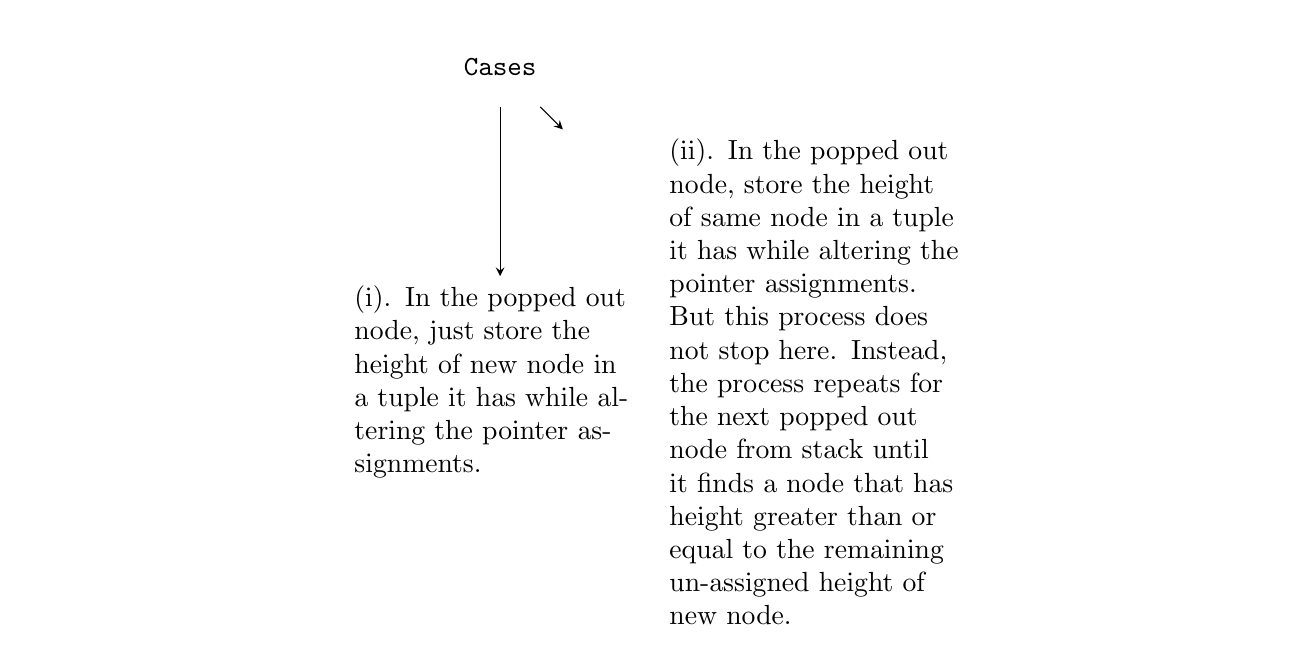
\begin{tikzpicture}[node distance=4cm]
				\node (cases)[parent]{\textbf{{\tt Cases}}};
				\node (case1)[child, below of=cases]{(i). In the popped out node, just store the height of new node in a tuple it has while altering the pointer assignments.};
				\node (case2)[child, right of=case1]{(ii). In the popped out node, store the height of same node in a tuple it has while altering the pointer assignments. But this process does not stop here. Instead, the process repeats for the next popped out node from stack until it finds a node that has height greater than or equal to the remaining un-assigned height of new node.};
				
				\draw [arrow] (cases) -- (case1);
				\draw [arrow] (cases) -- (case2);
			\end{tikzpicture}
			
			A similar process can be done for the successor node of new node to fix pointer assignments. This way we get rid of the possibility of multiple comparisons in {\tt find()} by just checking the counter of particular pointer in a tuple and directly descending counter levels down. 
			
			
		\end{solution}
\pagebreak
		
		\titledquestion{4.9*}[5]
		Explain how we can implement a version of a skiplist that implements the SSet interface, but also allows fast access to elements by rank. That is, it also supports the function $get(i)$, which returns the element whose rank is $i$ in $O(\log n)$ expected time. (The rank of an element $x$ in an SSet is the number of elements in the SSet that are less than $x$.)
		\begin{solution}
			We know that skiplist in its worst case operates with $log(n)$ complexity. In terms of Big-O notation, the skiplist has a default time complexity of $O(log(n))$. Hence, in this case, we need not worry about the logical algorithmic changes. Instead we alter the implementation to cater rank in it. This version of skiplist implementation will store the rank of every node with in itself along with its data value. This way, our {\tt get()} method will make decisions based on ranks instead of data values. Hence, leading to the access of elements in the $O(log(n))$ expected time. \\
			The question here arises that how will our algorithm decide the rank of newly formed node in the {\tt add()} process. The answer to this is very simple; just check the rank of predecessor node, add one to the rank of predecessor node. This way we get the rank of a new node. 
		\end{solution}
\pagebreak
		
		\titledquestion{4.14* (challenge)}[0]
		Using an {\tt SSet} as your underlying structure, design an application that reads a (large) text file and allows you to search, interactively, for any substring contained in the text. As the user types their query, a matching part of the text (if any) should appear as a result.
		
		\noindent\underline{Hint 1}: Every substring is a prefix of some suffix, so it suffices to store all suffixes of the text file.
		
		\noindent\underline{Hint 2}: Any suffix can be represented compactly as a single integer indi- cating where the suffix begins in the text.
		
		Test your application on some large texts, such as some of the books available at \href{http://www.gutenberg.org/}{Project Gutenberg}. If done correctly, your application will be very responsive; there should be no noticeable lag between typing keystrokes and seeing the results.
		\begin{solution}
		  % Write your solution here
		\end{solution}
\pagebreak
		
		\titledquestion{5.1}[5]
		A certain university assigns each of its students student numbers the first time they register for any course. These numbers are sequential integers that started at 0 many years ago and are now in the millions. Suppose we have a class of one hundred first year students and we want to assign them hash codes based on their student numbers. Does it make more sense to use the first two digits or the last two digits of their student number? Justify your answer.
		\begin{solution}
			The given scenario maps student numbers as sequential integers. Integers are the set of numbers in which every previous element is one less than its next element. In other words, every next element is one plus the previous element at the unit position with corresponding changes at the tenth, hundredth, thousandth positions and so on (if applicable). In this particular question where the number of students is $100$, the last two digits best serve the purpose because there exists a unique combination of digits for every value to be hashed. Hence, the answer is, last two digits. 
		\end{solution}
\pagebreak
		
		\titledquestion{5.2}
		Consider the hashing scheme in Section 5.1.1, and suppose $n = 2^d$ and $d \leq {w/2}$.
		\begin{parts}
		  \part[5] Show that, for any choice of the muliplier, z, there exists n values that all have the same hash code. (Hint: This is easy, and doesn’t require any number theory.)
		  \begin{solution}
		  	The answer to this question lies in the modulous operation. To show whether there exist $n$ values that all have the same hash code we assume a set $S$ whose cardinality is much larger than $2^d$ (i.e. a bigger domain). Following the formula of \underline{Multiplicative Hashing}, \begin{center} $h(x) = (z.x$ mod $2^w)$ div $2^{w-d}$ \end{center} let $x$ be any member of $S$ and for any choice of $z$ we apply the above formula to generate a hash code size $2w$ atmost (assuming that $z$ and $x$ are both $w$-bit). The $mod$ operation after multiplication truncates the larger code according to the size of the table. Following the pigeon-hole principle, we can show that there can be at least $n$ values which correspond to the same hash code because of truncation process as it maps multiple values to the same index in H-table because of $mod$ operation.
	  	  \end{solution}
  	  		
		    \part[5] Given the multiplier, z, describe n values that all have the same hash code. (Hint: This is harder, and requires some basic number theory.)
		  \begin{solution}
		  	Continuing the argument made in previous part, let $m$ be any number of the larger domain $S$ and for the sake of simplicity, let's assume that $m$ is either equal to $n$ or some multiple of $n$. Since $n$ is equal to the size of table and its $mod$ with the size of the table will always give us 0. The answer to mod will also be 0 for the multiples of $n$ ($2n$, $3n$, $4n$, ..., $n^{2}$) Hence corresponding to the same index (in this case, 0) in hash table. \\
		  	Similarly for $m=n+1$ and its n multiples, the hash code will be 1, and so on.\\ \\
		  	
		  	\underline{\textit{Note}: The assumption that $m=n$ is just for making the explanation simpler. It can always }\\ \underline{work for any other assumption.}
		  \end{solution}
		\end{parts}
\pagebreak
		
		\titledquestion{5.5}[10]
		Consider the following simplified version of the code for
		adding an element x to a LinearHashTable, which simply stores x in the first nil array entry it finds. Explain why this could be very slow by giving an example of a sequence of O(n) add(x), remove(x), and find(x) operations that would take on the order of $n^2$ time to execute. (For pseudocode refer to pg\# 125, Exercise 5.5).
		\begin{solution}
		  Assuming that the function {\tt hash(x)} in the pseudocode is not one of the best functions. Instead it is the type of hash function that generates the already occupied index time and again. If the function {\tt hash(x)} is a bad hash function and points to the same index frequently then in order to find the first $nil$ entry the function will need to iterate over the table until the time it finds the first nill entry. \\In order to visualise the process, let's assume that the hash function always generates the index 0. The first time it generates the index 0, the value gets stored. But the next time it generates the same index it will store the value at index 1. For $n$ values the function will iterate $1+2+3+ ... + n$ times in order to accomodate all the n values to a unique row in table which contained $nil$ in it. Summing up the number of iterations we have a total of ${n(n+1)/2}$ iterations; which leads to the asymptotic complexity of $O({n^2})$.\\
		  Now proving it for the sequence of {\tt add()} and {\tt remove()} operations, the current {\tt add\_slow()} function does not fill the entry of a row where $del$ exists. Hence, firstly the space complexity will rise much higher if {\tt remove()} is applied to hash table. Moreover in order to find the first $nil$ entry the function will have to iterate over the whole H-table but now with an extra over-head of iterating over the $del$ values.	Asympotically for multiple insertions and removals, the function will be of the cost of $O({n^2})$.\\ \\
		  \underline{\textit{Note: }Even if the {\tt hash(x)} function does not always points to the same index but assuming it to}\\ \underline{be a bad hash function it still points to the already occupied index. So asymptotically, the}\\ \underline{complexity will still be $O({n^2})$}.
		\end{solution}
\pagebreak
		
		\titledquestion{5.9}[10]
		Suppose you have an object made up of two w-bit integers, x and y. Suppose that the hash code for your object is defined by some deterministic function h(x, y) that produces a single w-bit integer. Prove that there exists a large set of objects that have the same hash code.
		\begin{solution}
			The answer to this question is somewhat related to the answer for Exercise 5.2. Suppose we have a table of dimension $d$ i.e. the total number of rows in a table are $2^d$. For any hash function, if $x$ and $y$ are hashed individually, we know that there exists a possibility of other w-bit integers also getting hashed to the same indices as that of $x$ and $y$ (talking in reference to mod operation and pigeon-hole principle). So if this argument is true then it follows that any complex object which consist of these two w-bit integers gets hashed to exactly the same index for multiple instances of $x$ and $y$. 
		\end{solution}
\pagebreak
		
		\titledquestion{5.10}[10]
		Let $p = 2^w - 1$ for some positive integer w. Explain why, for a positive integer x
		\begin{center}
			($x$ mod $2^w$) + ($x$ div $2^w$) $\equiv$ $x$ mod ($2^w - 1)$.
		\end{center}
		(This gives an algorithm for computing $x$ mod $(2^w - 1)$ by repeatedly setting until $x \leq 2^w - 1$.)
		\begin{solution}
			From the definition of congruency ($'\equiv'$ symbol) in $mod$ operation, we know that if we have, 
			\begin{center}
				$(b \equiv a)\%n$
			\end{center}
			then it means that $a-b$ is completely divisible by $n$. In other words, the remainder of $(a-b)/n$ turns out to be $0$ in this case.\\
			Mathematically, 
			\begin{center}
				$(a-b)\%n = 0$
			\end{center}
			The question here arises that why does this relation hold. The reason is fairly simple and addresses the division relationship of any number $p$ with any number $q-1$ and its successor $q$, given that $p \geq q$. The argument we are trying to establish here is shown below in mathematical notation. \\ \\
			Let $x$ be a number and $y$ be another number such that $x > y$ and $y = {2^w}$. Suppose $a$ and $b$ be the divident ($div$) and remainder ($mod$) respectively after dividing $x$ by $y$. Therefore, \begin{center}$y.a + b = x$\end{center}.
			The above equation can also be written as, 
			\begin{center}$(y-1).a + a + b = x$\\ $(y-1).a = x - a - b$\end{center}
			Therefore, the resultant value on R.H.S. is always divisible by $y-1$. Hence proved..
		\end{solution}
	
	\end{questions}

* - The question has been modified from the one in the book to exclude implementation. ``Design'' in a question here means to write pseudocode.

\end{document}